\documentclass{article}
\usepackage[mast]{lucky}

\title{3D Geometry}
\author{Dennis Chen}
\date{GQU}

\begin{document}
\maketitle

The idea is basically “figure out what matters, then only look there.”
\section{Techniques}
We assume basic competence in 3D Geometry. This means knowing all of the volume and surface area formulas.

\subsection{Cross-sections}
Sometimes it's possible to simplify a problem into 2 dimensions. This makes it much easier to visualize. \textbf{Do this whenever possible.}

\begin{defi}[Cross-section]
A cross-section of a solid is the intersection of the solid with a plane.
\end{defi}

You can also take cross-sections of a cube and a cone. The former is used sometimes in math competitions, and the latter produces a shape known as a \textit{conic}.

\begin{theo}[Cross-section of a Cube]
The cross-section of a cube can be a triangle, quadrilateral, pentagon, or hexagon.
\end{theo}

The heuristical reason this is true is because a cube has $6$ faces, and the plane can intersect the cube at any $6$ of those faces. It's not too hard to construct any polygon with less than $7$ sides.

Sometimes the entire problem is reduced significantly or just solved by taking the correct cross section.

\begin{exam}
Inside a cone of radius $5$ and height $12$ there is a sphere inscribed. What is its radius?
\end{exam}
\begin{sol}
Here is a walkthrough of the solution.
\begin{enumerate}
    \item Take a cross section through the apex of the cone perpendicular to the base.
    
    \item Now you have a triangle and its incircle. Finish with $[ABC]=rs.$
\end{enumerate}
\end{sol}

\begin{exam}[AMC 10A 2019/21]
A sphere with center $O$ has radius 6. A triangle with sides of length $15$, $15$, and $24$ is situated in space so that each of its sides are tangent to the sphere. What is the distance between $O$ and the plane determined by the triangle?
\end{exam}
\begin{sol}
Here is a walkthrough of the solution.
\begin{enumerate}
    \item This is not actually a 3D geometry problem.

    \item Take a cross section of the sphere with the triangle.
    
    \item Use $[ABC]=rs$ to figure out the radius of the cross-section.
    
    \item Finish with the Pythagorean Theorem.
\end{enumerate}
\end{sol}

\subsection{Pythagorean Theorem}
Here are some demonstrations of assorted Pythagorean Theorem techniques.

\begin{exam}
Consider unit cube $ABCDEFGH,$ where $ABCD$ and $EFGH$ are opposite faces and $AG,$ $BH,$ $CE,$ $DF$ are space diagonals. Find the area of triangle $AFH.$
\end{exam}

\begin{sol}
Note that $AF=FH=HA=\sqrt{2}$ by the Pythagorean Theorem, so the area is $\frac{(\sqrt{2})^2\sqrt{3}}{4}=\frac{\sqrt{3}}{2}.$
\end{sol}

\begin{exam}[AHSME 1996/9]
Triangle $PAB$ and square $ABCD$ are in perpendicular planes. Given that $PA = 3, PB = 4$ and $AB = 5$, what is $PD?$

\begin{center}
    \begin{asy}
pen ExamColor = rgb(240,200,200);
size(5cm);
    import olympiad;
    real r=sqrt(2)/2;
draw(origin--(8,0)--(8,-1)--(0,-1)--cycle);
draw(origin--(8,0)--(8+r, r)--(r,r)--cycle);
filldraw(origin--(-6*r, -6*r)--(8-6*r, -6*r)--(8, 0)--cycle, ExamColor, black);
filldraw(origin--(8,0)--(8,6)--(0,6)--cycle, ExamColor, black);
pair A=(6,0), B=(2,0), C=(2,4), D=(6,4), P=B+1*dir(-65);
draw(A--P--B--C--D--cycle);
dot(A^^B^^C^^D^^P);
label("$A$", A, dir((4,2)--A));
label("$B$", B, dir((4,2)--B));
label("$C$", C, dir((4,2)--C));
label("$D$", D, dir((4,2)--D));
label("$P$", P, dir((4,2)--P));
    \end{asy}
\end{center}
\end{exam}

\begin{sol}
Note that $\angle PAD=90^{\circ},$ so $PD=\sqrt{PA^2+DA^2}=\sqrt{3^2+5^2}=\sqrt{34}.$
\end{sol}

For problems with tangent spheres, remember the following fact.
\begin{fact}[Tangency Point is Collinear with Centers]
If two spheres with centers $O_1,O_2$ are tangent at $T,$ then $O_1,O_2,T$ are collinear.
\end{fact}
This implies the following corollary.
\begin{fact}[Distance Between Centers]
Say two spheres $\Gamma_1,\Gamma_2$ with centers $O_1,O_2$ and radii $r_1,r_2$ are tangent at $T.$ Then
\[\begin{cases}
O_1O_2=r_1+r_2 \text{ if } \Gamma_2 \text{ is externally tangent to } \Gamma_1 \\
O_1O_2=r_1-r_2 \text{ if } \Gamma_2 \text{ is internally tangent to } \Gamma_1.
\end{cases}\]
\end{fact}
Using this in conjunction with the Pythagorean Theorem is enough to solve almost all problems with tangent spheres.
\begin{exam}[AMC 12A 2004/22]
Three mutually tangent spheres of radius $1$ rest on a horizontal plane. A sphere of radius $2$ rests on them. What is the distance from the plane to the top of the larger sphere?
\end{exam}
\begin{sol}
Let's label some points. Let the centers of the unit spheres be $O_1,O_2,O_3,$ let the center of the sphere of radius $2$ be $O,$ and let the foot of the perpendicular from $O$ to $O_1O_2O_3$ be $P.$ Note that $O_1O_2O_3$ is parallel to the horizontal plane with a distance of $1.$

Note that $\triangle O_1O_2O_3$ is equilateral with side length $2,$ and by symmetry, $P$ must be the center. Thus $PO_1=\frac{2\sqrt{3}}{3}.$ Since $OO_1=3$ by Fact $2,$ $OP=\sqrt{OO_1^2-PO_1^2}=\sqrt{3^2-(\frac{2\sqrt{3}}{3})^2}=\frac{\sqrt{69}}{3}.$

Since the distance from $P$ to the horizontal plane is $1$ and the tip of the sphere with radius $2$ is $2$ above $O,$ the answer is $1+2+\frac{\sqrt{69}}{3}=3+\frac{\sqrt{69}}{3}.$
\end{sol}
\begin{center}
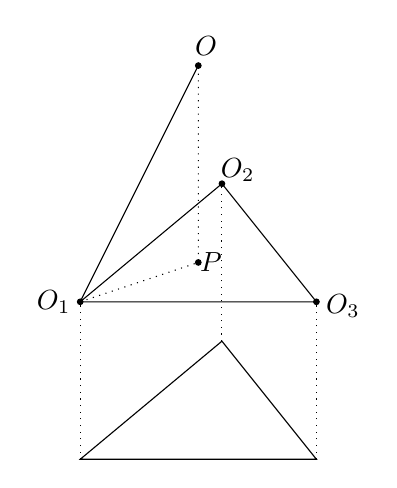
\begin{tikzpicture}
    \draw (0,0)--(1.8,1.5)--(3,0)--cycle;
    \draw (0,2)--(1.8,3.5)--(3,2)--cycle;
    \draw [dotted] (0,0)--(0,2);
    \draw [dotted] (1.8,1.5)--(1.8,3.5);
    \draw [dotted] (3,0)--(3,2);
    \draw [dotted] (0,2)--(1.5,2.5)--(1.5,5);
    \draw (1.5,5)--(0,2);
    \node at (0,2) [anchor=east] {$O_1$};
    \node at (2,3.4) [anchor=south] {$O_2$};
    \node at (3,1.95) [anchor=west] {$O_3$};
    \node at (1.4,2.5) [anchor=west] {$P$};
    \node at (1.6,5) [anchor=south] {$O$};
    \filldraw (0,2) circle (1pt);
    \filldraw (1.8,3.5) circle (1pt);
    \filldraw (3,2) circle (1pt);
    \filldraw (1.5,2.5) circle (1pt);
    \filldraw (1.5,5) circle (1pt);
\end{tikzpicture}
\end{center}

Notice that the entire solution was essentially just doing the correct setup and using the Pythagorean Theorem.

%\section{Tetrahedron Centers}

\pagebreak

\section{Problems}

\minpt{32}

\psetquote{Does `read the mood' mean he should be a person that suits everyone? If so, then you're the ones with a few screws loose!}{Yugami-kun Has No Friends}

\begin{prob}[AMC 12B 2005/16]{2}
Eight spheres of radius 1, one per octant, are each tangent to the coordinate planes. What is the radius of the smallest sphere, centered at the origin, that contains these eight spheres?
\end{prob}

\begin{prob}[]{2}
A pyramid has a square base $ABCD$ and vertex $E$. The area of square $ABCD$ is $196$, and the areas of $\triangle ABE$ and $\triangle CDE$ are $105$ and $91$, respectively. What is the volume of the pyramid?
\end{prob}

\begin{prob}[]{2}
Consider two externally tangent spheres $\Gamma_1$ and $\Gamma_2$ with radii $12,r,$ and consider cylinder $\Omega$ with radius $16$ and height $25.$ If $\Gamma_1$ is internally tangent to a base and the circumference of $\Omega$ and $\Gamma_2$ is internally tangent to the opposite base and the circumference of $\Omega,$ find $r.$
\end{prob}

\begin{req}[AMC 10B 2018/10]{2}
In the rectangular parallelepiped shown, $AB$ = $3$, $BC$ = $1$, and $CG$ = $2$. Point $M$ is the midpoint of $\overline{FG}$. What is the volume of the rectangular pyramid with base $BCHE$ and apex $M$?
\end{req}

\begin{center}
    \begin{asy}
    import olympiad;
    size(6cm);
pair A = origin;
pair B = (4.75,0);
pair E1=(0,3);
pair F = (4.75,3);
pair G = (5.95,4.2);
pair C = (5.95,1.2);
pair D = (1.2,1.2);
pair H= (1.2,4.2);
pair M = ((4.75+5.95)/2,3.6);
draw(E1--M--H--E1--A--B--E1--F--B--M--C--G--H);
draw(B--C);
draw(F--G);
draw(A--D--H--C--D,dashed);
label("$A$",A,SW);
label("$B$",B,SE);
label("$C$",C,E);
label("$D$",D,W);
label("$E$",E1,W);
label("$F$",F,SW);
label("$G$",G,NE);
label("$H$",H,NW);
label("$M$",M,N);
dot(A);
dot(B);
dot(E1);
dot(F);
dot(G);
dot(C);
dot(D);
dot(H);
dot(M);
label("3",A/2+B/2,S);
label("2",C/2+G/2,E);
label("1",C/2+B/2,SE);
    \end{asy}
\end{center}

\begin{prob}[AIME 1984/9]{2}
In tetrahedron $ABCD$, edge $AB$ has length 3 cm. The area of face $ABC$ is $15\mbox{cm}^2$ and the area of face $ABD$ is $12 \mbox { cm}^2$. These two faces meet each other at a $30^\circ$ angle. Find the volume of the tetrahedron in $\mbox{cm}^3$.
\end{prob}

\begin{prob}[AMC 10A 2013/22]{3}
Six spheres of radius $1$ are positioned so that their centers are at the vertices of a regular hexagon of side length $2$. The six spheres are internally tangent to a larger sphere whose center is the center of the hexagon. An eighth sphere is externally tangent to the six smaller spheres and internally tangent to the larger sphere. What is the radius of this eighth sphere?
\end{prob}

\begin{prob}[AMC 12A 2005/22]{3}
A rectangular box $P$ is inscribed in a sphere of radius $r$. The surface area of $P$ is 384, and the sum of the lengths of its 12 edges is 112. What is $r$?
\end{prob}

\begin{prob}[AIME I 2020/6]{3}
A flat board has a circular hole with radius $1$ and a circular hole with radius $2$ such that the distance between the centers of the two holes is $7.$ Two spheres with equal radii sit in the two holes such that the spheres are tangent to each other. The square of the radius of the spheres is $\tfrac{m}{n},$ where $m$ and $n$ are relatively prime positive integers. Find $m+n.$
\end{prob}

\begin{prob}[AMC 12B 2004/19]{3}
A truncated cone has horizontal bases with radii $18$ and $2$. A sphere is tangent to the top, bottom, and lateral surface of the truncated cone. What is the radius of the sphere?
\end{prob}

\begin{prob}[AIME II 2020/7]{4}
Two congruent right circular cones each with base radius $3$ and height $8$ have axes of symmetry that intersect at right angles at a point in the interior of the cones a distance $3$ from the base of each cone. A sphere with radius $r$ lies inside both cones. The maximum possible value for $r^2$ is $\frac mn$, where $m$ and $n$ are relatively prime positive integers. Find $m+n$.
\end{prob}

\begin{prob}[AHSME 1996/28]{4}
On a $4\times 4\times 3$ rectangular parallelepiped, vertices $A$, $B$, and $C$ are adjacent to vertex $D$. Find the distance from $D$ to plane $ABC$.
\end{prob}

\begin{prob}[AIME I 2001/12]{6}
A sphere is inscribed in the tetrahedron whose vertices are $A = (6,0,0), B = (0,4,0), C = (0,0,2),$ and $D = (0,0,0).$ The radius of the sphere is $m/n,$ where $m$ and $n$ are relatively prime positive integers. Find $m + n.$
\end{prob}

\begin{prob}[AIME I 2013/7]{6}
A rectangular box has width $12$ inches, length $16$ inches, and height $\frac{m}{n}$ inches, where $m$ and $n$ are relatively prime positive integers. Three faces of the box meet at a corner of the box. The center points of those three faces are the vertices of a triangle with an area of $30$ square inches. Find $m+n$.
\end{prob}

\begin{req}[NARML 10]{9}
Three mutually tangent spheres with radii of $1$ are tangent to a table, and a cone is tangent to all three spheres with its tip oriented towards the table. If the cone has height $\sqrt{2}$ and its tip is $\tfrac{3+\sqrt{3}}{3}$ units above the table, compute the radius of the cone.
\end{req}

\begin{prob}[AIME II 2016/14]{13}
Equilateral $\triangle ABC$ has side length $600$. Points $P$ and $Q$ lie outside the plane of $\triangle ABC$ and are on opposite sides of the plane. Furthermore, $PA=PB=PC$, and $QA=QB=QC$, and the planes of $\triangle PAB$ and $\triangle QAB$ form a $120^{\circ}$ dihedral angle (the angle between the two planes). There is a point $O$ whose distance from each of $A,B,C,P,$ and $Q$ is $d$. Find $d$.
\end{prob}

\begin{prob}[AIME II 2017/15]{13}
Tetrahedron $ABCD$ has $AD=BC=28$, $AC=BD=44$, and $AB=CD=52$. For any point $X$ in space, define $f(X)=AX+BX+CX+DX$. The least possible value of $f(X)$ can be expressed as $m\sqrt{n}$, where $m$ and $n$ are positive integers, and $n$ is not divisible by the square of any prime. Find $m+n$.
\end{prob}
\end{document}